\documentclass[11pt,a4paper]{article}
\usepackage[margin=2.2cm]{geometry}
\usepackage{amsmath}
\usepackage{graphicx,booktabs,longtable,array,xcolor,hyperref,pgfgantt,enumitem,float,caption}
\hypersetup{colorlinks=true,linkcolor=black,urlcolor=blue}
\graphicspath{{../diagrams/}{../screenshots/}}


\newcommand{\StudentName}{Ridhikanta Sarkar Sumit}
\newcommand{\StudentID}{IT24045}
\newcommand{\CourseName}{SEPM}
\newcommand{\Supervisor}{Dr. Ziaur Rahman}
\newcommand{\RepoURL}{https://github.com/sumitnoob/SEPM-project}
%%%%%%%%%%%%%%%%%%%%%%%%%%%%%%%%%%%%%%%%%
\title{\textbf{MessFinder}\\[2pt]\large A Smart Mess Recommendation Platform for New Students\\[4pt]\normalsize Final Capstone Project -- Part I: Proposal and Prototyping}
\author{\StudentName \\ Student ID: \StudentID \\ Course: \CourseName \\ Supervisor: \Supervisor}
\date{\today}
\begin{document}
\maketitle
\begin{abstract}
Every year, thousands of new students arrive on campus and must find a \emph{mess} (a subscription-based meal service) that matches their budget, food habits and location. Today this is done through word of mouth, which is slow, unreliable and biased. \textbf{MessFinder} is a web platform where students enter their preferences and receive a ranked list of suitable messes, backed by menus and honest reviews from current students. Mess owners manage their listings and subscription requests, and an administrator verifies listings and moderates content. This document presents the proposal, schedule, UML models and a working prototype.
\end{abstract}
\tableofcontents\newpage

\section{Introduction}
\subsection{Problem Statement}
New students have no reliable way to compare messes. Information about price, distance, hygiene and menu quality is scattered across personal contacts and social media posts. As a result students often choose poorly, pay more than necessary, or must switch after a month, while good small messes struggle to reach new customers.

\subsection{Objectives}
\begin{enumerate}[nosep]
\item Provide a single searchable directory of verified messes near campus.
\item Rank messes automatically by how well they match each student's preferences.
\item Show weekly menus, prices and multi-criteria reviews (food, hygiene, service, value).
\item Let students request a subscription and owners approve or reject it online.
\item Give administrators tools to verify listings and moderate reviews.
\end{enumerate}

\subsection{Scope}
\textbf{In scope:} user accounts for three roles, mess listing and menu management, search/filter, preference-based ranking, reviews and ratings, subscription requests, admin moderation, a responsive web interface.\\
\textbf{Out of scope (future work):} online payment, delivery tracking, native mobile apps, AI-based menu analysis.

\subsection{Stakeholders}
\begin{tabular}{@{}p{3cm}p{12cm}@{}}\toprule
\textbf{Stakeholder} & \textbf{Interest}\\\midrule
Students & Find a suitable, affordable, hygienic mess quickly.\\
Mess owners & Reach more customers; manage menu, prices and subscribers.\\
Administrator & Keep listings genuine and reviews fair.\\
University / hall authority & Better student welfare and food-quality visibility.\\
Project supervisor & Evaluate scope, quality and documentation.\\\bottomrule
\end{tabular}

\section{Requirements}
\subsection{Functional Requirements}
\begin{longtable}{@{}p{1.2cm}p{13.5cm}@{}}\toprule
\textbf{ID} & \textbf{Requirement}\\\midrule\endhead
FR1 & Users shall register and log in as Student, Mess Owner or Admin.\\
FR2 & Students shall set preferences: maximum budget, maximum distance, food type, meals per day.\\
FR3 & The system shall search and filter messes and rank them by a match score.\\
FR4 & The system shall display mess details and the weekly menu.\\
FR5 & Students shall compare two or more messes side by side.\\
FR6 & Students shall submit reviews with ratings for food, hygiene, service and value.\\
FR7 & Students shall request a subscription; owners shall approve or reject it.\\
FR8 & Owners shall create and edit their mess profile, menu and prices.\\
FR9 & Admins shall approve new mess listings and remove inappropriate reviews.\\\bottomrule
\end{longtable}

\subsection{Non-Functional Requirements}
\begin{tabular}{@{}p{3cm}p{12cm}@{}}\toprule
\textbf{Attribute} & \textbf{Requirement}\\\midrule
Performance & Search results shall load in under 2 seconds for up to 500 messes.\\
Usability & A new student shall find a mess within 3 minutes without training; mobile-friendly layout.\\
Security & Passwords hashed; role-based access control; input sanitised against XSS and SQL injection.\\
Reliability & Availability of at least 99\% during admission season.\\
Maintainability & Modular, object-oriented code that mirrors the class diagram.\\\bottomrule
\end{tabular}

\subsection{Recommendation Logic}
Each approved mess receives a match score out of 100 for a student's preferences:
\[ \text{Score} = S_{price}(35) + S_{distance}(25) + S_{food}(20) + S_{meals}(10) + \tfrac{\text{rating}}{5}\times 10 \]
Price and distance earn full points within the student's limits and lose points proportionally beyond them. Food type earns points on an exact match (or ``Any''), meals on meeting the requested count.

\section{Feasibility and Risk Analysis}
\textbf{Technical:} uses mature, free technologies. \textbf{Economic:} negligible cost; free hosting tiers suffice for the pilot. \textbf{Operational:} owners need only a simple form; students use a browser.
\begin{longtable}{@{}p{4.2cm}p{1.8cm}p{9cm}@{}}\toprule
\textbf{Risk} & \textbf{Level} & \textbf{Mitigation}\\\midrule\endhead
Few owners join at launch & High & Personally onboard 10--15 nearby messes; admin can enter listings on their behalf.\\
Fake or biased reviews & Medium & Only students may review; admin moderation; one review per student per mess.\\
Scope creep & Medium & Agile backlog with strict sprint goals; extras go to future work.\\
Outdated menus/prices & Medium & Show ``last updated'' date; reminders to owners.\\
Schedule slip & Medium & Buffer in final sprint; prioritise must-have features first.\\\bottomrule
\end{longtable}

\section{Process Model, Schedule and Deliverables}
\subsection{Chosen Process Model: Agile (Scrum)}
Requirements such as filters and ranking weights will change after students try the system, so an iterative, feedback-driven model fits better than Waterfall. The project runs as \textbf{six two-week sprints (12 weeks)}, each ending with a working increment and a review.

\subsection{Sprint Plan}
\begin{tabular}{@{}llp{9.3cm}@{}}\toprule
\textbf{Sprint} & \textbf{Weeks} & \textbf{Goal}\\\midrule
0 & 1--2 & Requirements, proposal, UML design, prototype\\
1 & 3--4 & Database schema, authentication, mess listing and menu management\\
2 & 5--6 & Search, filters, preference-based ranking, comparison view\\
3 & 7--8 & Reviews and ratings, subscription workflow\\
4 & 9--10 & Admin moderation, UI polish, system testing\\
5 & 11--12 & User acceptance test with students, deployment, final report\\\bottomrule
\end{tabular}

\subsection{Gantt Chart}
\begin{figure}[H]\centering\small
\begin{ganttchart}[hgrid,vgrid={*{12}{dotted}},x unit=0.78cm,y unit title=0.55cm,y unit chart=0.55cm,
title height=1,bar/.append style={fill=green!55!black},milestone/.append style={fill=red!70!black},
bar label font=\footnotesize,milestone label font=\footnotesize,title label font=\footnotesize]{1}{12}
\gantttitle{Week}{12}\\
\gantttitlelist{1,...,12}{1}\\
\ganttbar{Requirements \& proposal}{1}{2}\\
\ganttbar{UML design \& prototype}{1}{2}\ganttmilestone{}{2}\\
\ganttbar{Database \& authentication}{3}{4}\\
\ganttbar{Mess \& menu management}{3}{4}\ganttmilestone{}{4}\\
\ganttbar{Search, filter \& ranking}{5}{6}\\
\ganttbar{Comparison view}{6}{6}\ganttmilestone{}{6}\\
\ganttbar{Reviews \& ratings}{7}{8}\\
\ganttbar{Subscription workflow}{7}{8}\ganttmilestone{}{8}\\
\ganttbar{Admin moderation}{9}{9}\\
\ganttbar{Testing \& UI polish}{9}{10}\ganttmilestone{}{10}\\
\ganttbar{User acceptance test}{11}{11}\\
\ganttbar{Deployment \& final report}{11}{12}\ganttmilestone{}{12}
\end{ganttchart}
\caption{Project Gantt chart (12 weeks, 6 sprints; red markers are milestones M1--M6, listed in the table below).}
\end{figure}

\subsection{Milestones and Deliverables}
\begin{tabular}{@{}lcp{4.2cm}p{6.2cm}@{}}\toprule
\textbf{ID} & \textbf{Week} & \textbf{Milestone} & \textbf{Deliverables}\\\midrule
M1 & 2 & Proposal and design approved & Proposal, UML diagrams, Gantt chart, prototype\\
M2 & 4 & Core data and accounts ready & Database schema, login, mess/menu CRUD\\
M3 & 6 & Recommendation engine working & Search, filters, ranking, comparison page\\
M4 & 8 & Social and booking features & Reviews, ratings, subscription workflow\\
M5 & 10 & System tested & Admin tools, test report, bug fixes\\
M6 & 12 & Final release & Deployed system, user manual, final report, demo\\\bottomrule
\end{tabular}

\section{Resources and Tools}
\begin{tabular}{@{}p{3.5cm}p{11.5cm}@{}}\toprule
Team & 1 student developer (analyst, designer, developer, tester); supervisor as product owner.\\
Technology & Python 3, Flask/Django (full system), SQLite then MySQL/PostgreSQL, HTML/CSS/JS.\\
Design & Graphviz / draw.io for UML; \LaTeX{} for documentation.\\
Management & Git and GitHub (version control, issues as backlog), GanttProject / pgfgantt.\\
Budget & Approx.\ 0 BDT development cost (free tiers); optional domain \& hosting about 1{,}500 BDT/year.\\\bottomrule
\end{tabular}

\section{System Design (UML and Related Diagrams)}
\subsection{Data Flow Diagram}
\begin{figure}[H]\centering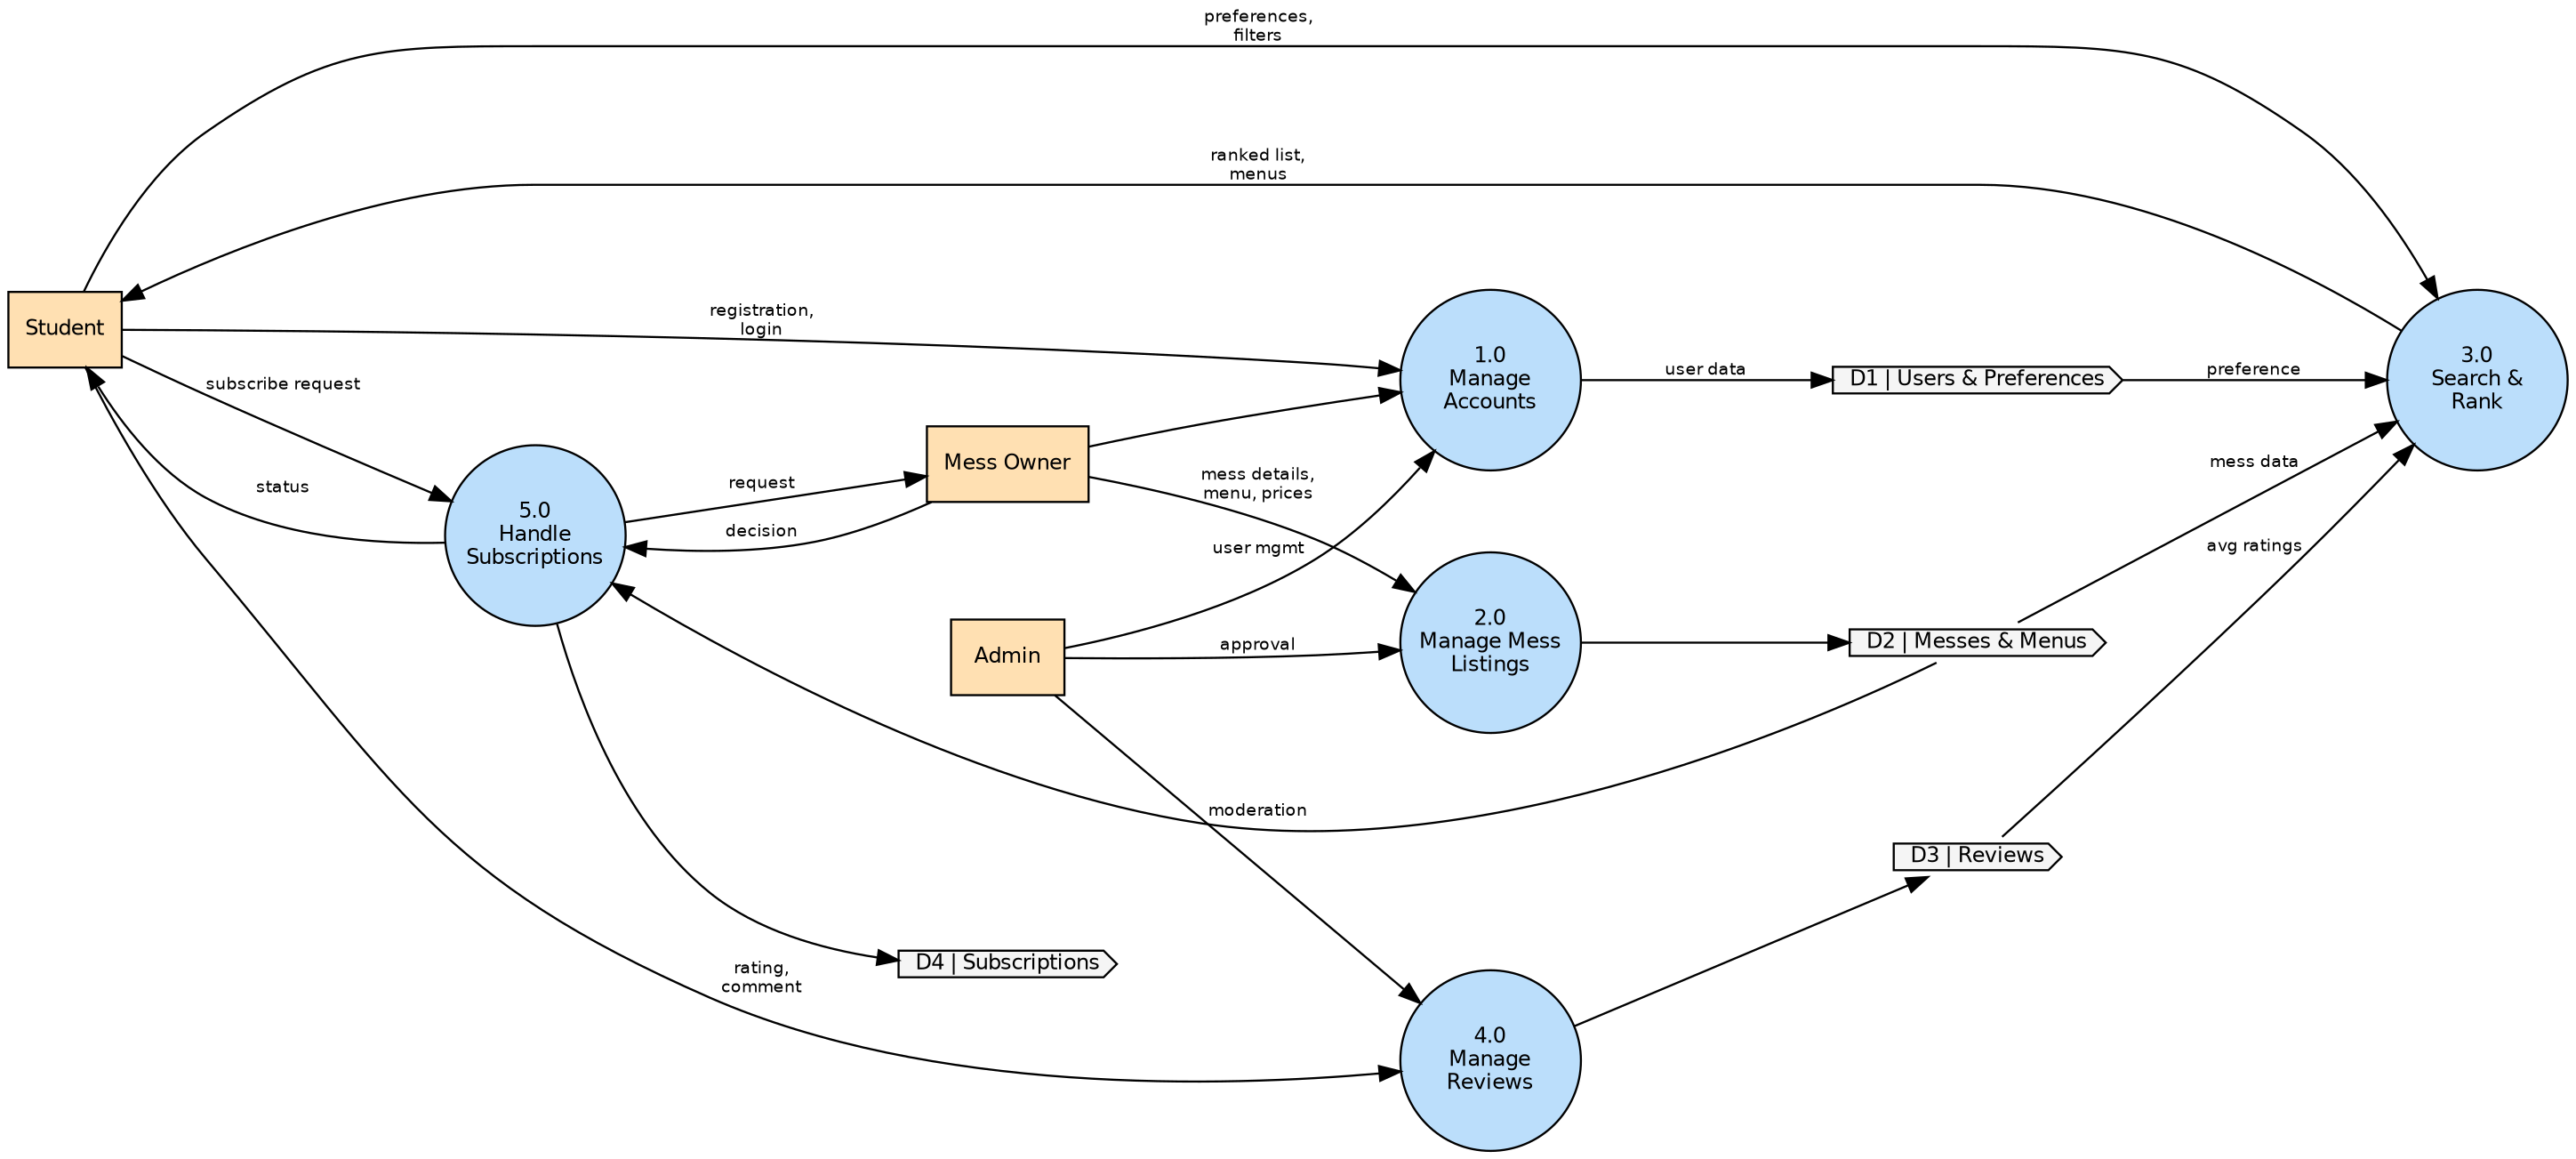
\includegraphics[width=\linewidth]{dfd.png}\caption{Level-1 Data Flow Diagram: five processes, four data stores.}\end{figure}
\subsection{Use Case Diagram}
\begin{figure}[H]\centering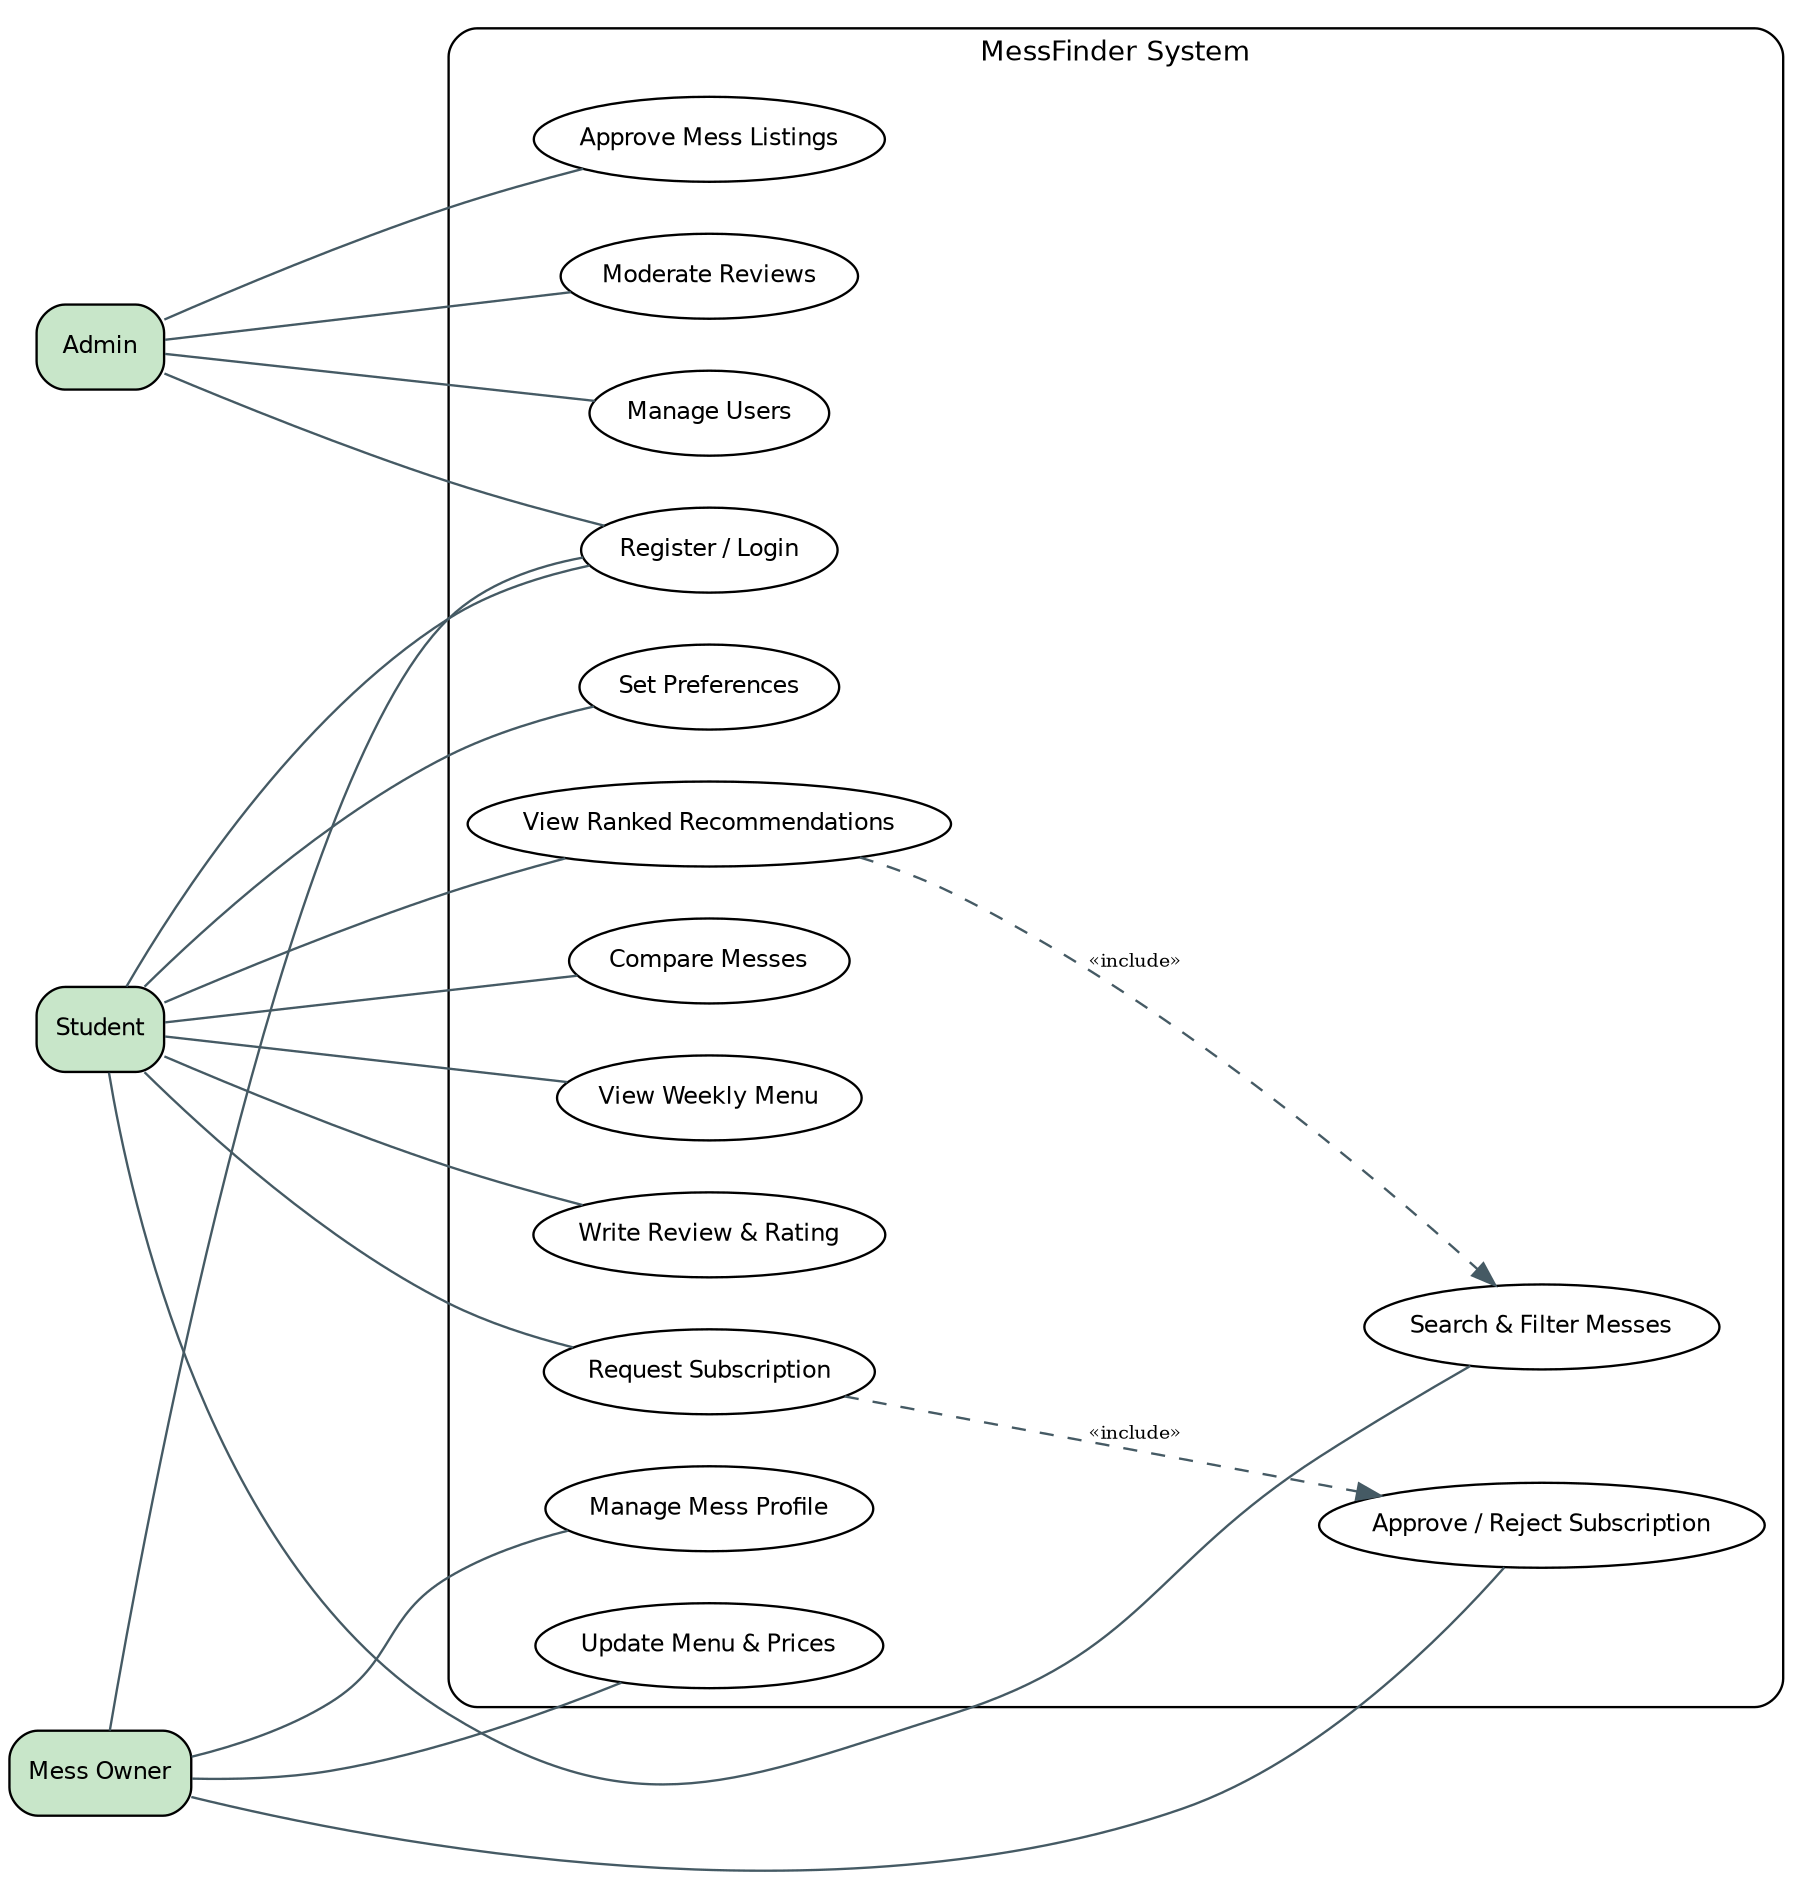
\includegraphics[width=0.95\linewidth]{use_case.png}\caption{Use case diagram for Student, Mess Owner and Admin.}\end{figure}
\subsection{Activity Diagram}
\begin{figure}[H]\centering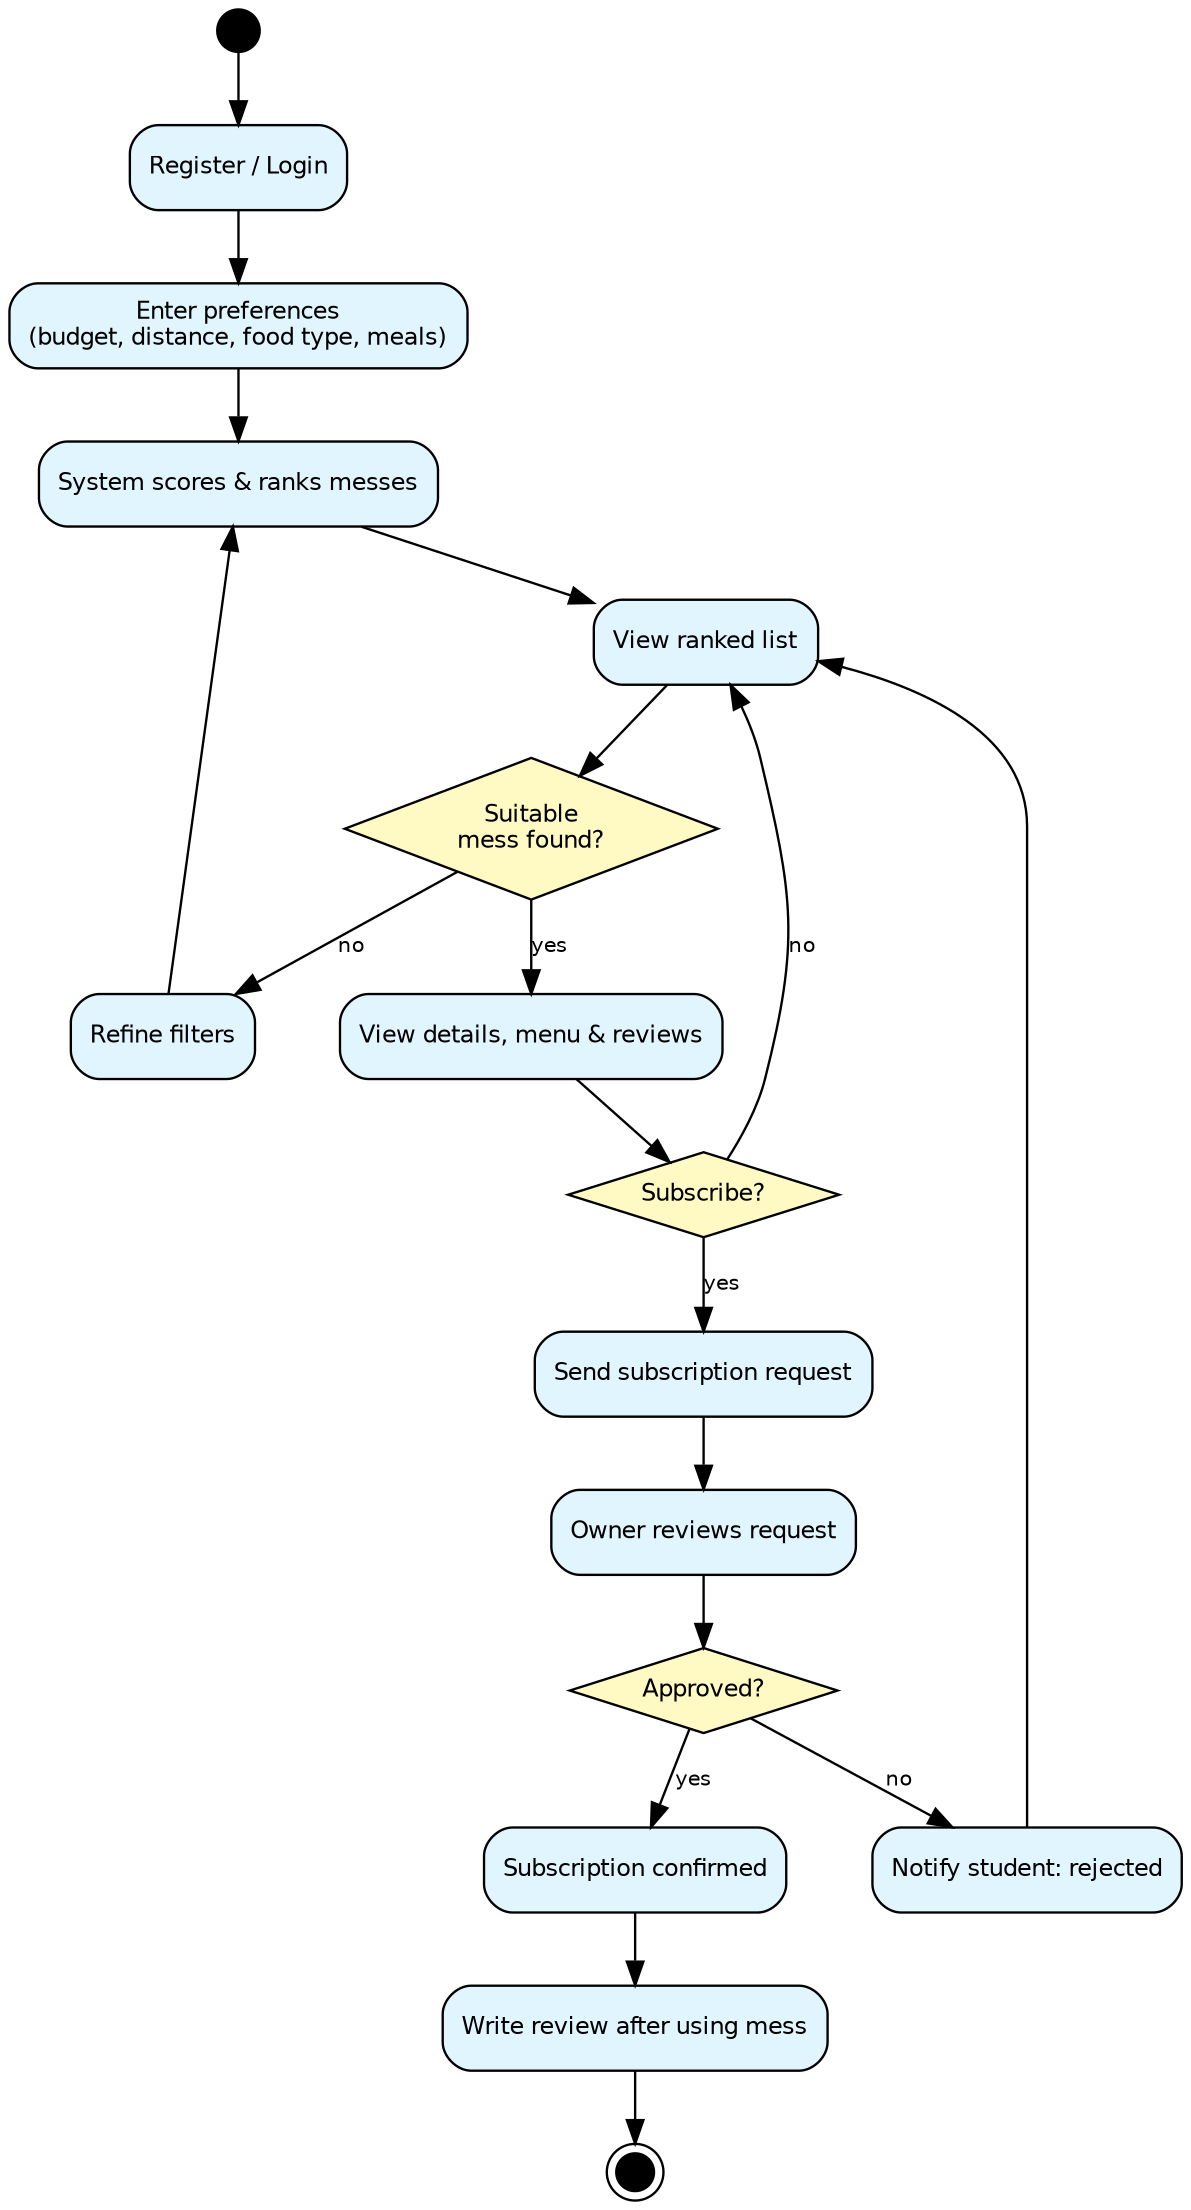
\includegraphics[height=0.62\textheight]{activity.png}\caption{Activity diagram: student finds and subscribes to a mess.}\end{figure}
\subsection{Entity Relationship Diagram}
\begin{figure}[H]\centering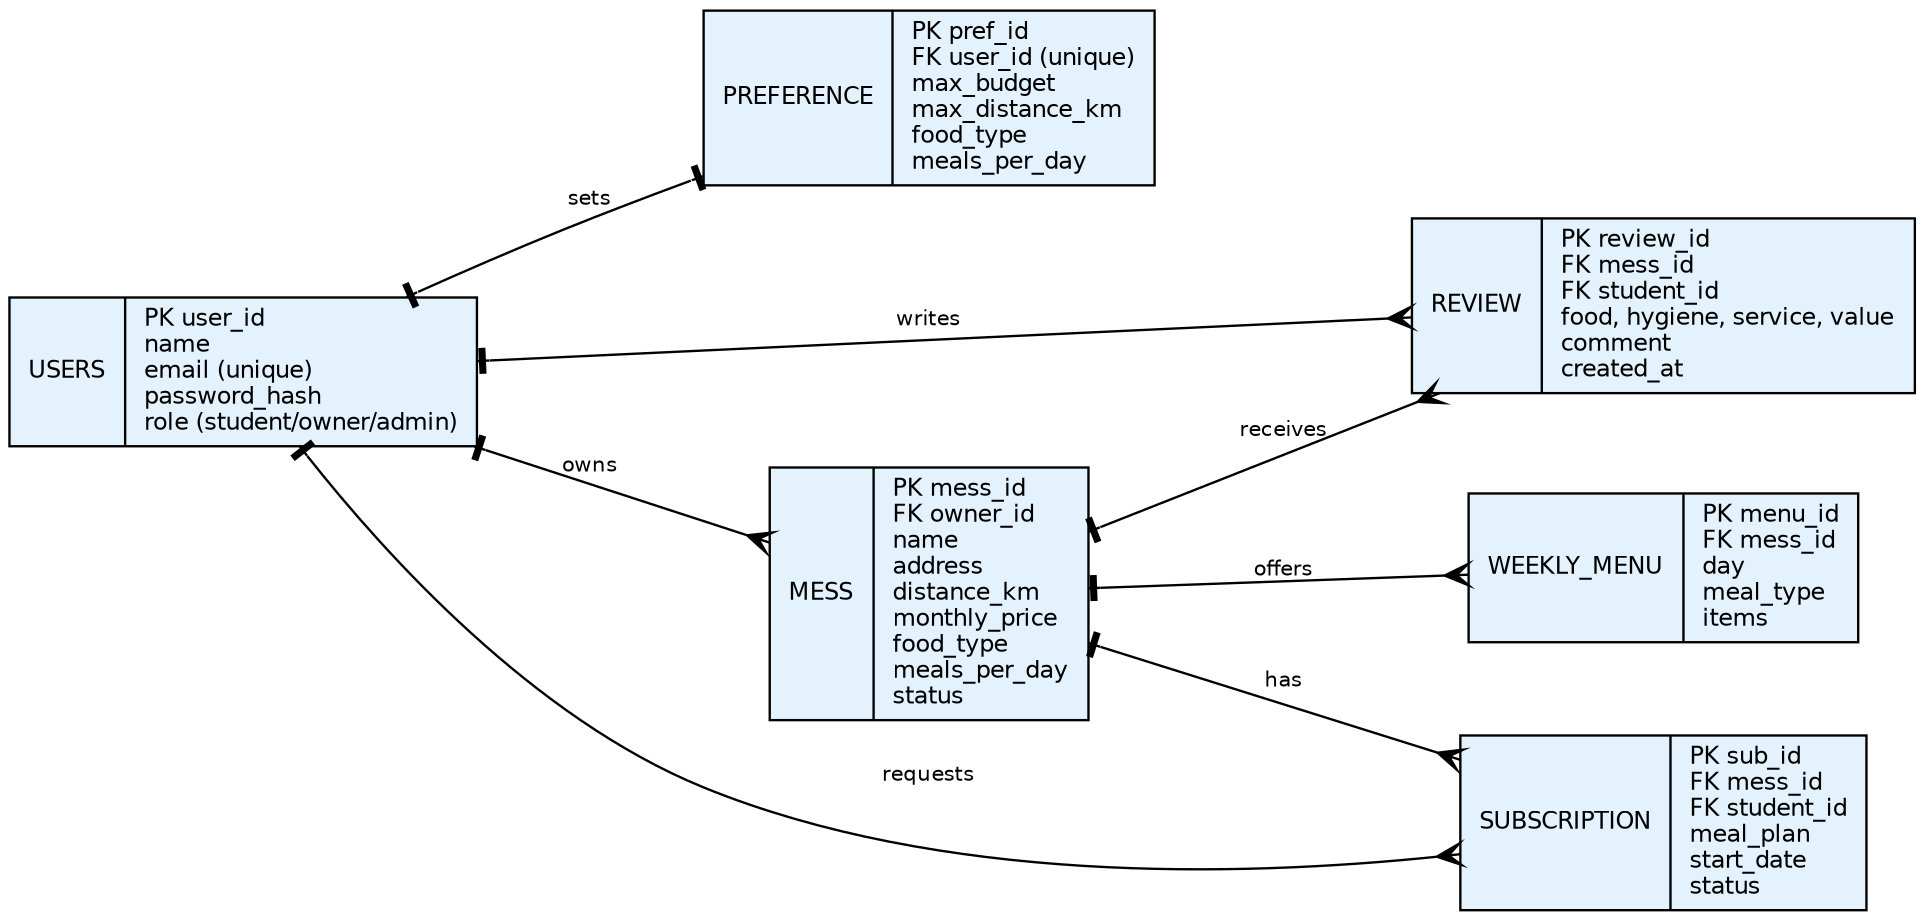
\includegraphics[width=\linewidth]{erd.png}\caption{ER diagram of the MessFinder database (crow's foot notation).}\end{figure}
\subsection{Class Diagram}
\begin{figure}[H]\centering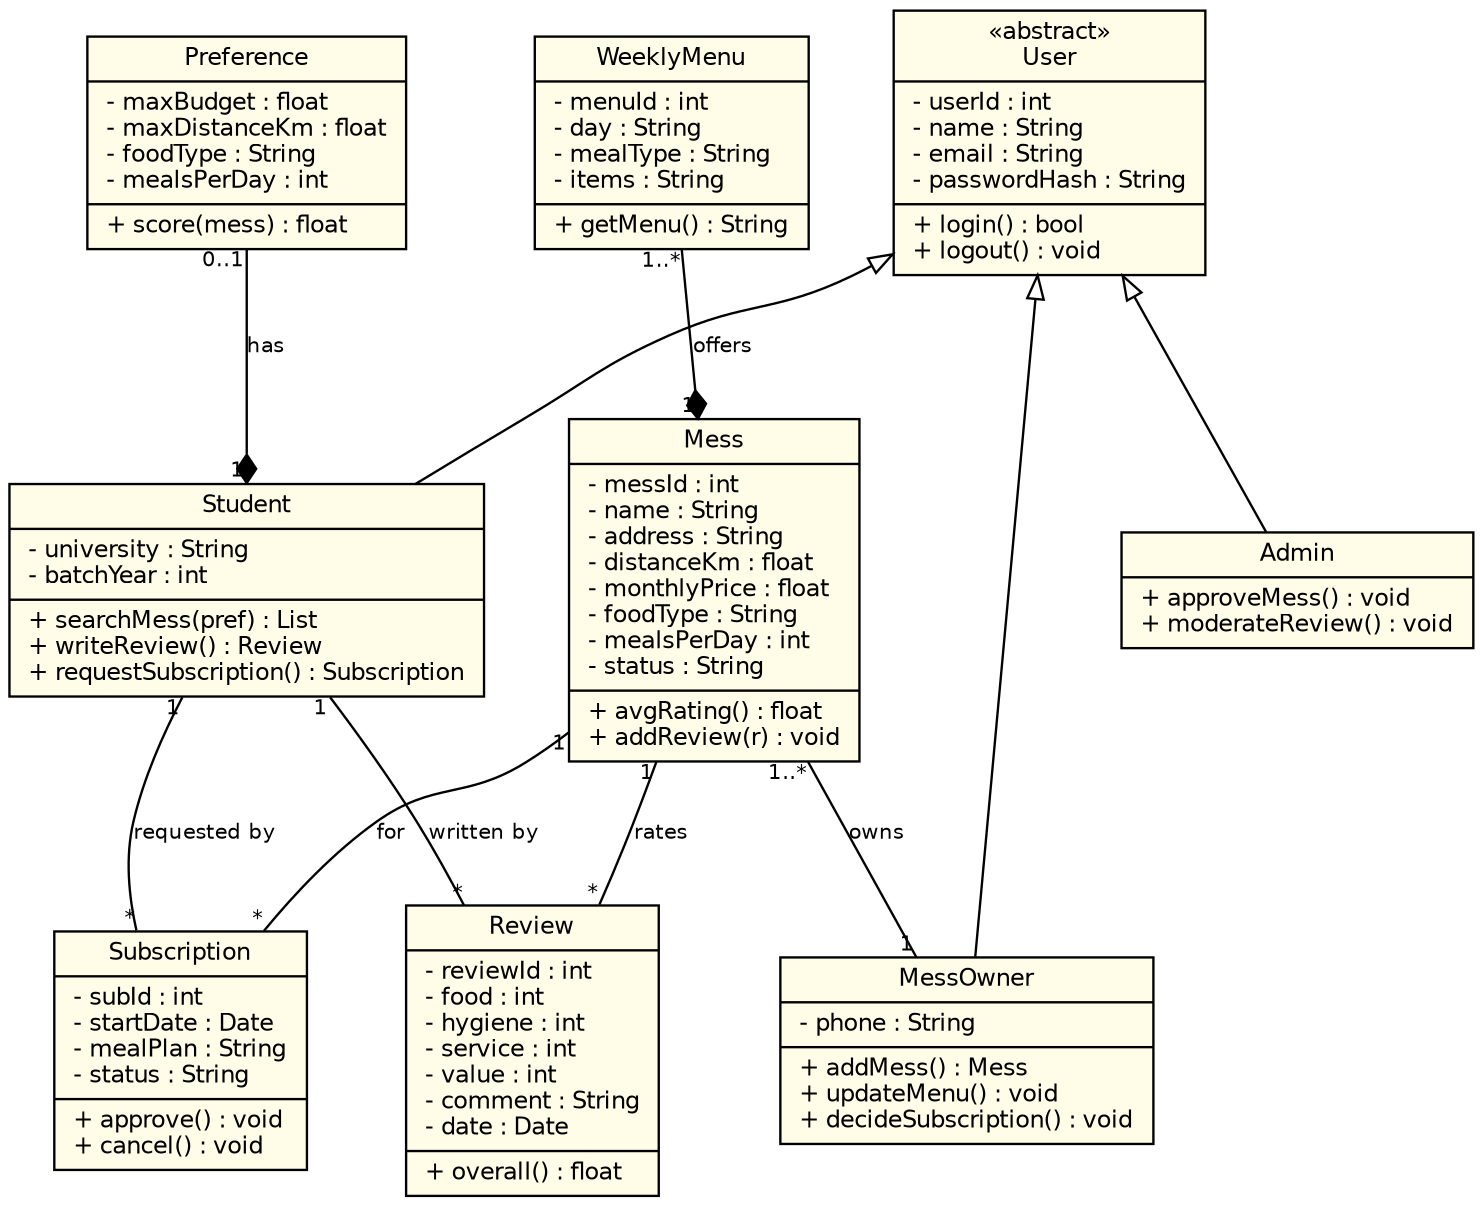
\includegraphics[width=\linewidth]{class_diagram.png}\caption{Class diagram: 9 classes with inheritance, composition and associations.}\end{figure}
\subsection{Object Diagram}
\begin{figure}[H]\centering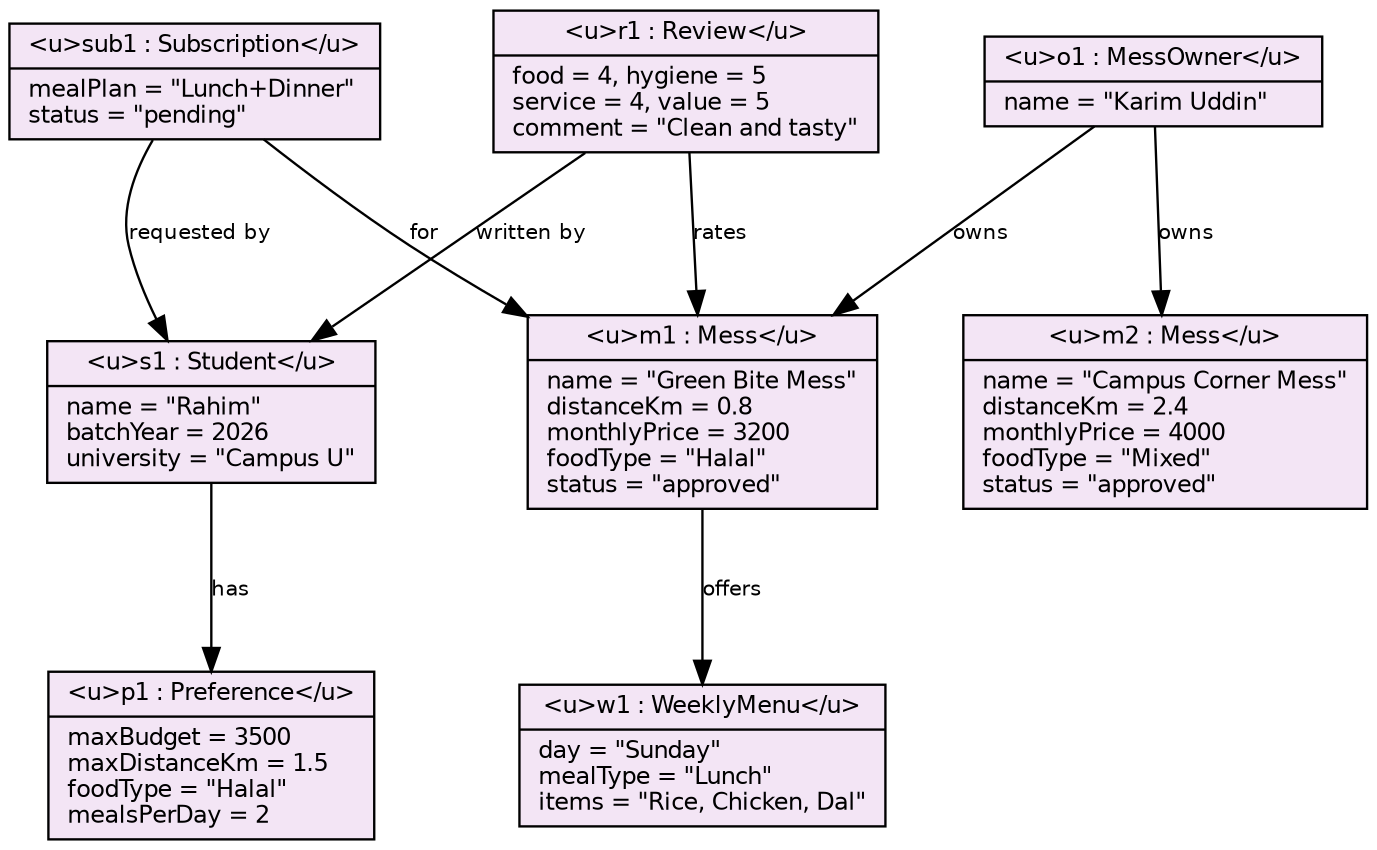
\includegraphics[width=\linewidth]{object_diagram.png}\caption{Object diagram: a snapshot of runtime objects for one student's search.}\end{figure}

\section{Prototype}
The prototype (folder \texttt{prototype/}) is a working web interface written in Python (standard library only). It implements nine classes from the class diagram in \texttt{models.py}: \texttt{User}, \texttt{Student}, \texttt{MessOwner}, \texttt{Admin}, \texttt{Mess}, \texttt{WeeklyMenu}, \texttt{Review}, \texttt{Subscription} and \texttt{Preference}. Run \texttt{python3 app.py} and open \texttt{http://localhost:8000}.
\begin{itemize}[nosep]
\item \textbf{Home:} preference form and ranked list with match percentage.
\item \textbf{Mess page:} details, weekly menu, reviews, review form, subscription request.
\item \textbf{Demo approval link:} simulates the owner approving a request.
\end{itemize}

\subsection{Screenshots}
\begin{figure}[H]\centering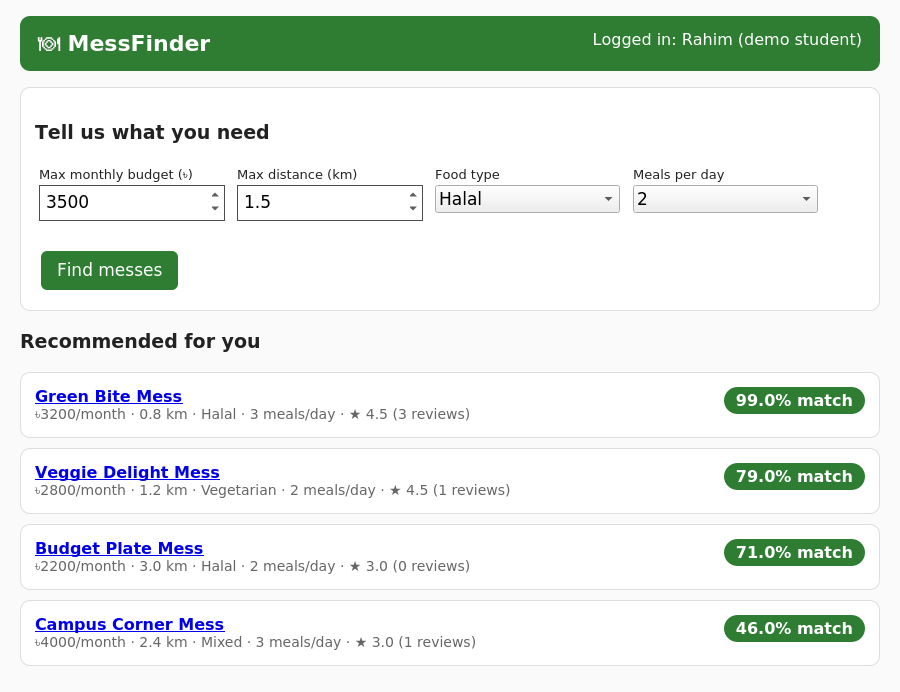
\includegraphics[width=0.85\linewidth]{home_ranked.png}\caption{Home page: preference form and ranked recommendations with match percentage.}\end{figure}
\begin{figure}[H]\centering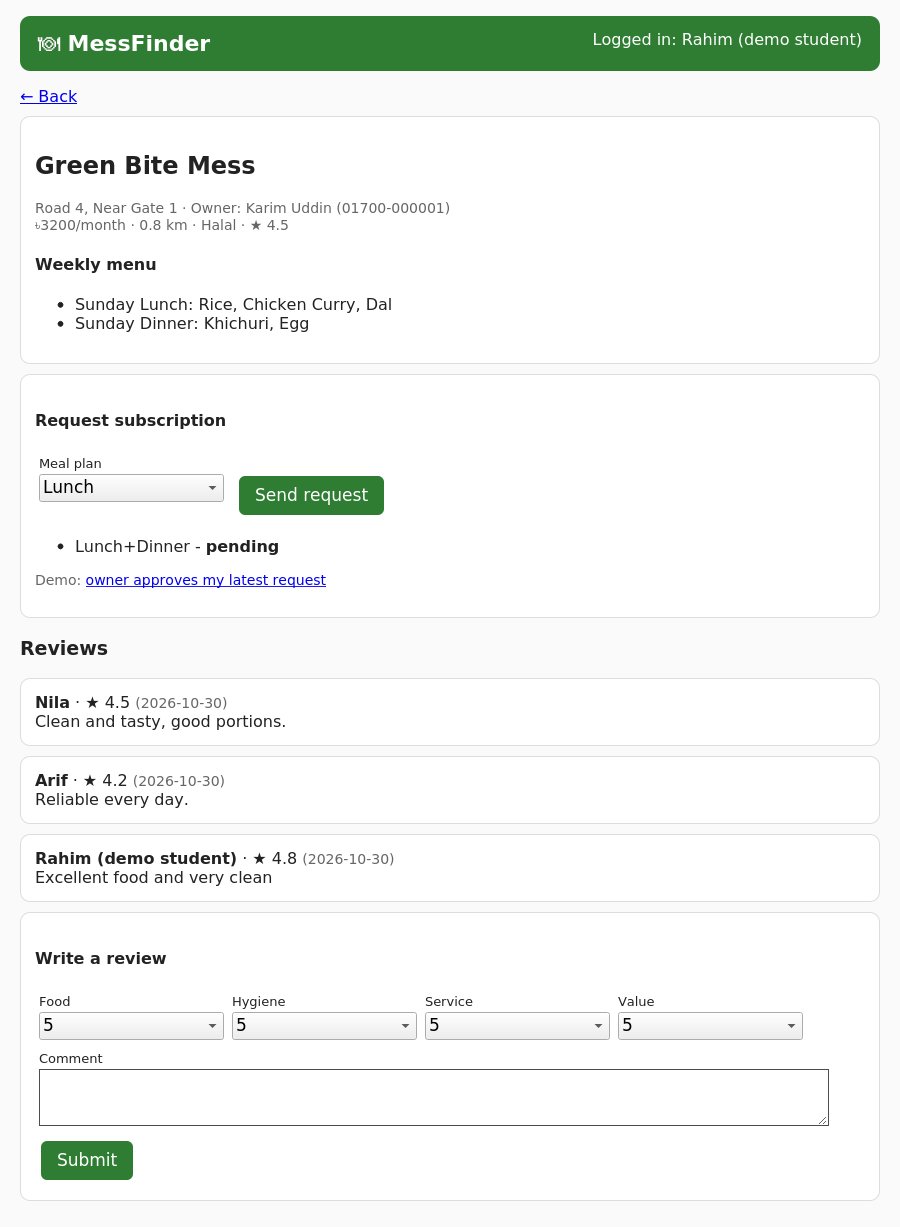
\includegraphics[width=0.85\linewidth]{mess_detail.png}\caption{Mess page: details, weekly menu, subscription request and reviews.}\end{figure}

\subsection{Class-to-Code Mapping}
\begin{tabular}{@{}p{3.5cm}p{11.5cm}@{}}\toprule
\textbf{Class} & \textbf{Implemented behaviour in \texttt{models.py}}\\\midrule
User, Student, MessOwner, Admin & Inheritance; \texttt{login()}, \texttt{search\_mess()}, \texttt{write\_review()}, \texttt{request\_subscription()}, \texttt{add\_mess()}, \texttt{decide\_subscription()}, \texttt{approve\_mess()}, \texttt{moderate\_review()}\\
Preference & \texttt{score(mess)} -- the 0--100 match score\\
Mess & \texttt{avg\_rating()}, \texttt{add\_review()}\\
WeeklyMenu & \texttt{get\_menu()}\\
Review & \texttt{overall()} -- mean of four ratings\\
Subscription & \texttt{approve()}, \texttt{cancel()}\\\bottomrule
\end{tabular}

\section{Testing Plan}
Ten automated unit tests already exist in \texttt{prototype/test\_models.py} (run \texttt{python3 -m unittest -v}; all pass) covering scoring, ranking, reviews, subscriptions and admin actions. Planned next: integration tests for the web workflows; usability testing with at least 10 new students; and security checks for input handling and role access.

\section{Conclusion}
MessFinder solves a real, recurring problem for new students with a feasible scope, a clear Agile plan and a design fully modelled in UML. The prototype already demonstrates the core idea: preference-based ranking of messes backed by menus, reviews and subscriptions.

\vspace{1em}\noindent\textbf{Repository:} \url{\RepoURL}
\end{document}
